\documentclass[11pt]{article}

\usepackage[english]{babel}
\usepackage[T1]{fontenc}
\usepackage[utf8x]{inputenc}

\usepackage{appendix}
\usepackage{cprotect}
\usepackage{listings}
\usepackage{float}
\usepackage[margin=2cm]{geometry}
\usepackage{graphicx}
\usepackage{underscore}

\lstset{
    tabsize=3,
    breakatwhitespace=true,
    breaklines=true,
    frame=simple
}

\title{Lab1 - FPGA Router}
\author{Matthew Walker - 999540475 - walker82}
\date{\today}

%TODO HPBBWL for each circuit
%TODO compare snapped vs not snapped
%TODO program flow

\begin{document}

\maketitle

\section{Results}
\begin{table}[ht]
\centering\begin{tabular}{ c *2r}
\hline\hline
Circuit & As Solved & After Final Legalization \\
\hline
cct1 & 133.15 & 146 \\
cct2 & 1376.63 & 1443 \\
cct3 & 9651.9 & 10414 \\
cct4 & 30959.2 & 32610 \\
\hline\hline
\end{tabular}
\caption{Half-perimeter-bounding-box wire lengths. \label{tab:hpbbwl}}
\end{table}

\section{Approach}


\section{Program Flow}

\clearpage
\appendix
\section*{Appendix}

\section{Result Plots}\label{app:result-plots}
\begin{figure}[H]
\centering
\includegraphics[clip, viewport=213 280 443 510, width=7cm]{assets/lab2/cct1-legalized.ps}
\cprotect\caption{\small\verb|anaplace --circuit data/anaplace/cct1.txt --graphics|}
\end{figure}

\begin{figure}[H]
\centering
\includegraphics[clip, viewport=176 247 468 539, width=11cm]{assets/lab2/cct2-legalized.ps}
\cprotect\caption{\small\verb|anaplace --circuit data/anaplace/cct2.txt --graphics|}
\end{figure}

\begin{figure}[H]
\centering
\includegraphics[clip, viewport=171 244 480 548, width=\linewidth]{assets/lab2/cct3-legalized.ps}
\cprotect\caption{\small\verb|anaplace --circuit data/anaplace/cct3.txt --graphics|}
\end{figure}
\begin{figure}[H]
\centering
\includegraphics[clip, viewport=196 269 454 523, width=\linewidth]{assets/lab2/cct4-legalized.ps}
\cprotect\caption{\small\verb|anaplace --circuit data/anaplace/cct4.txt --graphics|}
\end{figure}

\end{document}
